\documentclass[main.tex]{subfiles}

\begin{document}
\sloppy

\section{Primi Tasks}\label{sec:Primi Tasks}
Come spiegato nell'introduzione, il tirocinio consiste in un primo periodo di \say{training} in cui si risolvono piccoli bug e vengono svolti piccoli task per prendere confidenza con il progetto. In questa sezione si passerà in rassegna ai primi task svolti esaminando e commentando la soluzione trovata. Questo passaggio è fondamentale in quanto, approcciandosi per la prima volta a nuove tecnologie su cui è costruito il progetto, o ne fa utilizzo, bisogna familiarizzarci prima di riuscire a lavorare autonomamente. Le tecnologie in questione sono \say{Docker} (un popolare software libero progettato per eseguire processi informatici in ambienti isolabili, minimali e facilmente distribuibili chiamati container, con l'obiettivo di semplificare i processi di deployment di applicazioni software\cite{docker}), git (software per il controllo di versione distribuito) e OpenAPI (specifica per file di interfaccia leggibili dalle macchine per descrivere, produrre, consumare e visualizzare servizi web RESTful).

\subsection{Re-design groups API}
Il task, come spiegato in figura \ref{fig:redesign-api-task}, chiede di riprogettare le API per entrare e uscire da un gruppo in quanto richiedono parametri ridondanti ed è necessario conoscere se l'utente è autenticato nell'app oppure no per usare l'API corretta. Infatti nel primo caso bisognerà usare l'API \say{/groups/\{groupid\}/members/\{userid\}}, nel secondo invece \say{/groups/\{groupid\}/phones/\{phoneid\}} mostrate nelle figure \ref{fig:redesign-api-swagger-phone-old} e \ref{fig:redesign-api-swagger-user-old}.
\begin{figure}[H]
    \centering
    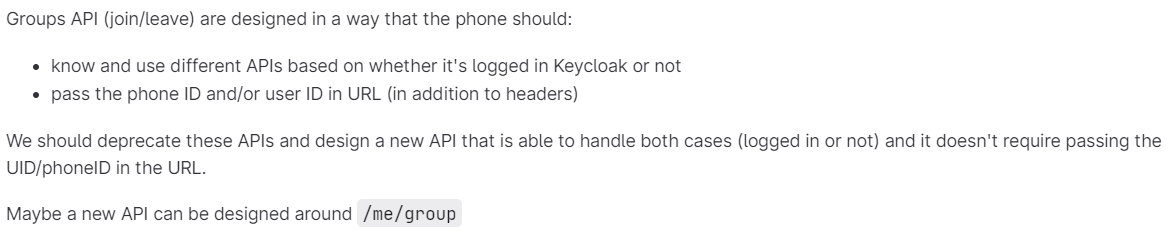
\includegraphics[width=1\linewidth]{img/redesign-api-task/redesign-api-task.png}
    \caption{Re-design groups API task}
    \label{fig:redesign-api-task}
\end{figure}

\begin{figure}[H]
    \centering
    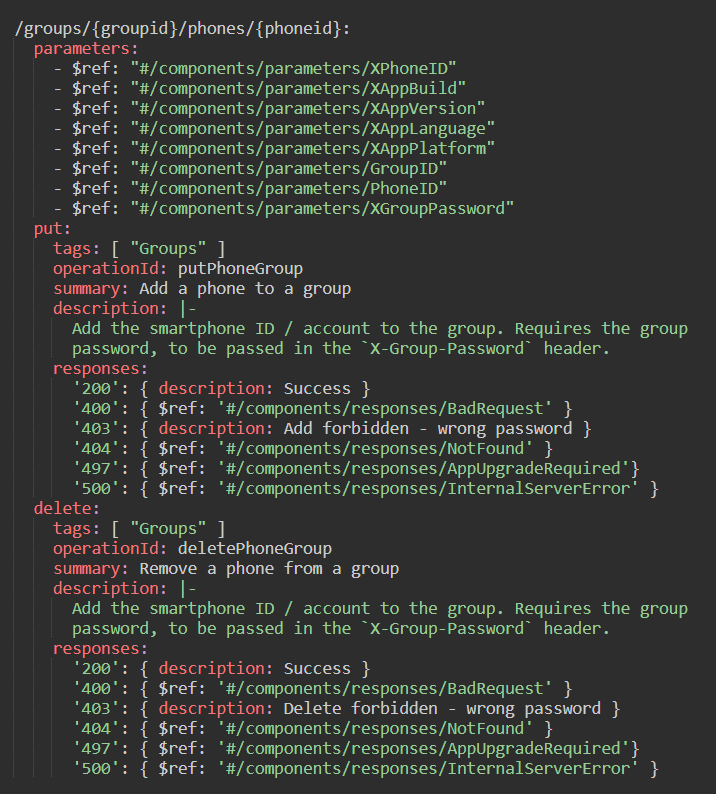
\includegraphics[width=1\linewidth]{img/redesign-api-task/redesign-api-swagger-phone-old.PNG}
    \caption{Documentazione API che aggiunge ed elimina un telefono da un gruppo}
    \label{fig:redesign-api-swagger-phone-old}
\end{figure}
\begin{figure}[H]
    \centering
    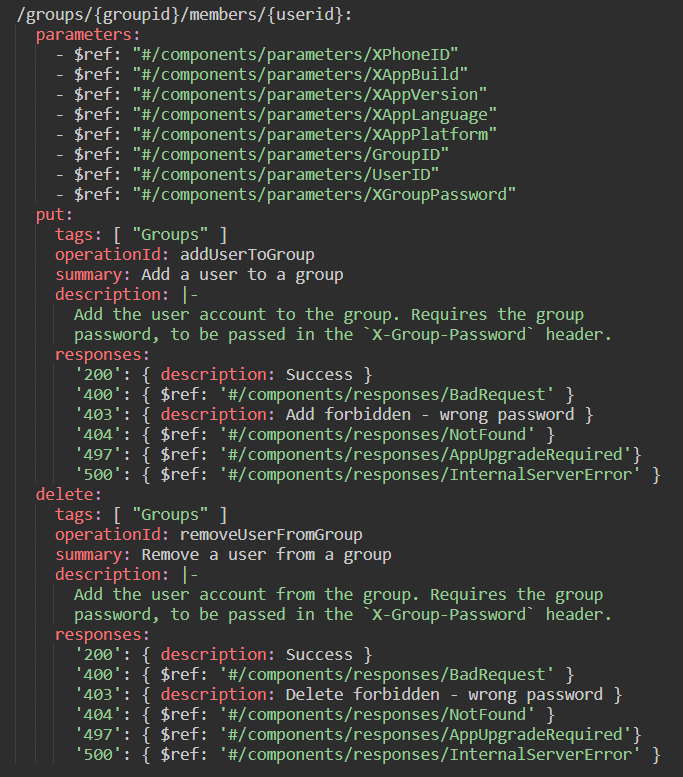
\includegraphics[width=1\linewidth]{img/redesign-api-task/redesign-api-swagger-user-old.PNG}
    \caption{Documentazione API che aggiunge ed elimina un utente registrato da un gruppo}
    \label{fig:redesign-api-swagger-user-old}
\end{figure}
\subsubsection{Cos'è un gruppo}\label{sec: gruppo}
Nel progetto SeismoCloud è stata aggiunta la funzionalità di chat/community. Un gruppo, dal momento in cui in passato venivano svolti progetti con istituti scolastici, serviva per creare un insieme di sensori associati a una determinata scuola; al momento i gruppi vengono utilizzati per fini statistici. Volendo, però, creare delle community nel progetto, in futuro un gruppo diventerà anche una \emph{chat room} in cui gli utenti che fanno parte dello stesso istituto scolastico avranno la possibilità di entrare, immettendo la password corretta, ed uscire. Per entrare nel gruppo non è necessaria l'autenticazione, basta aver solo installato l'applicazione; infatti all'installazione verrà assegnato un \emph{phoneid} per utilizzare le API.\newline

\subsubsection{Risoluzione task}
Per prima cosa bisogna trovare un corretto design per le nuove API. Come veniva suggerito nel task sono state costruite sotto \say{/me/group}, in quanto logicamente sotto \say{/me} vi sono tutte le API che coinvolgono l'utente; inoltre, sono stati spostati dall'header alcuni parametri in modo da passare un unico \emph{JSON} che verrà processato dal server. L'utilizzo del \emph{JSON} aumenta la mantenibilità delle API in quanto si potranno facilmente aggiungere e rimuovere parametri con piccole modifiche. Lato server basterà modificare la struttura per processare il \emph{JSON}, mentre per il client servirà solo di cambiare i parametri inviati.\newline
Trovato il corretto design per le nuove API non resta che svilupparle, deprecando le vecchie, e scriverne la nuova documentazione.
\begin{figure}[H]
    \centering
    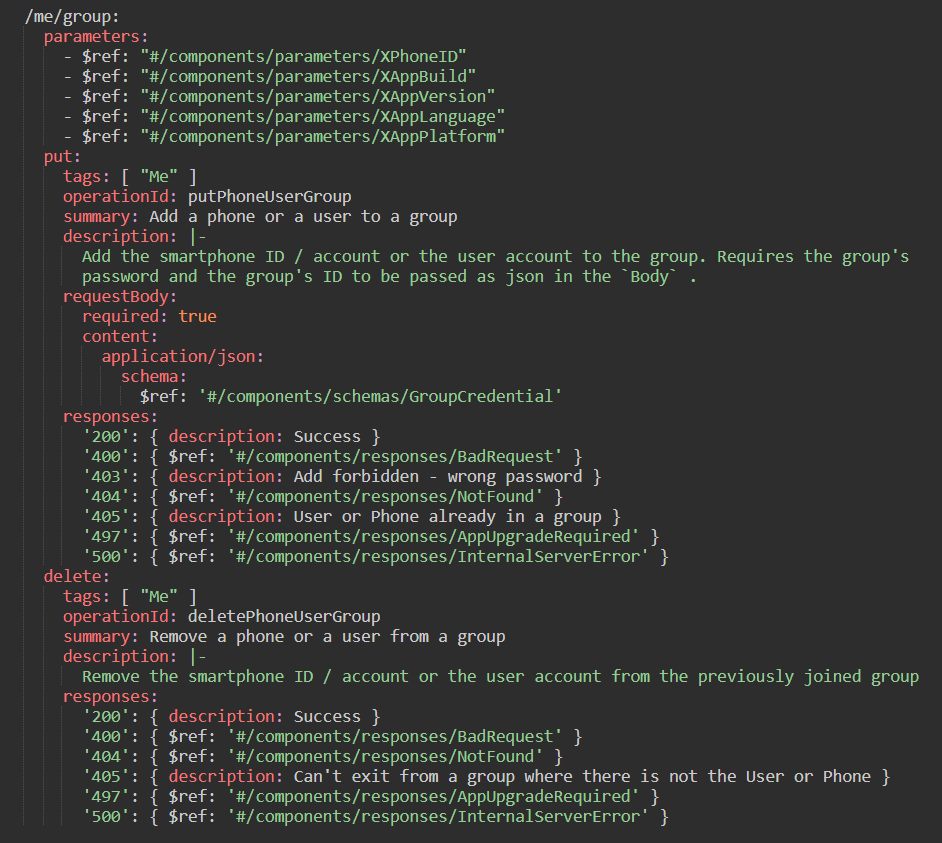
\includegraphics[width=1\linewidth]{img/redesign-api-task/redesign-api-swagger-user-phone-new.PNG}
    \caption{Documentazione API /me/group}
    \label{fig:redesign-api-swagger-user-phone-new}
\end{figure}
Per sviluppare le API è servito semplicemente controllare, tramite i parametri nell'header, se il client fosse autenticato e quindi comportarsi di conseguenza. Nel primo caso all'interno dell'header è presente un \say{user id} che identifica univocamente l'utente, nel secondo invece è solo presente il \say{phone id} che identifica univocamente il telefono con cui si esegue la richiesta. Il \say{phone id} è presente sia con che senza autenticazione. Una volta convalidata l'autenticità della richiesta bisogna distinguere i due casi:
\begin{itemize}
    \item \textbf{Richiesta di accesso a un gruppo} (PUT), accertarsi che l'utente non faccia già parte di un gruppo e che la password sia corretta. La richiesta, se sono presenti degli errori nell'esecuzione, va rigettata con la corretta risposta HTTP, oppure accettarla e inserire un nuovo record all'interno del database ritornando la risposta HTTP 200 (OK).
    \item \textbf{Richiesta di rimozione da un gruppo} (DELETE), accertarsi che l'utente faccia parte di un gruppo. La richiesta, se sono presenti degli
errori nell’esecuzione, va rigettata con la corretta risposta HTTP, oppure accettarla e rimuovere il record dal database ritornando la risposta HTTP 200 (OK).
\end{itemize}
\newpage

\subsection{Add API for link of the group}
Il task, come spiegato in figura \ref{fig:add-link-issue}, consiste nel creare un \say{\emph{join ID}} per entrare all'interno dei gruppi (vedi \say{Cos'è un gruppo \ref{sec: gruppo}}) oppure condividerlo ad altri utenti, migliorando la loro esperienza nell'app semplificandone l'accesso.

\begin{figure}[H]
    \centering
    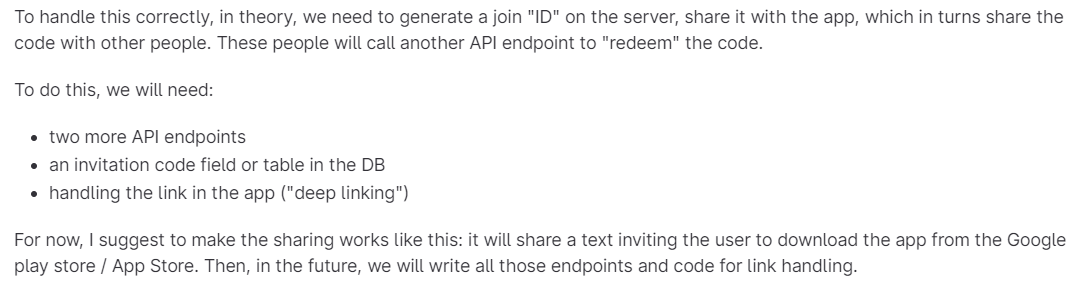
\includegraphics[width=1\linewidth]{img/add-link-task/add-link-issue.PNG}
    \caption{Task add API for link of the group}
    \label{fig:add-link-issue}
\end{figure}

\subsubsection{Risoluzione del task}
Per risolvere il task è stato necessario: progettare i nuovi endpoints API, prima scrivendo la documentazione per poi passare all'implementazione, aggiornare il database mantenendo la retro compatibilità, trovare un modo per generare degli identificativi univoci sicuri per gli \emph{invitation id}.

\subsubsection{Security design}
Gli \emph{invitation id} sono degli identificativi univoci a cui è associato un singolo gruppo. E' importante creare l'identificativo il più sicuro possibile, in quanto permette di poter entrare in un gruppo bypassando la password.\newline
La prima idea è stata quella di usare lo stesso identificativo del gruppo, ovvero un numero intero incrementale (vedere figura \ref{fig:invitation-first}), come \emph{invitation id}; ciò comporterebbe un grave problema di sicurezza, in quanto sarà possibile effettuare una chiamata all'API \say{/groups/} (figura \ref{fig:groups}), la quale ritorna un JSON con la lista di strutture contenti ID, nome e la descrizione di ogni gruppo esistente. Perciò sarà possibile entrare facilmente in ogni gruppo.
\begin{figure}[H]
    \centering
    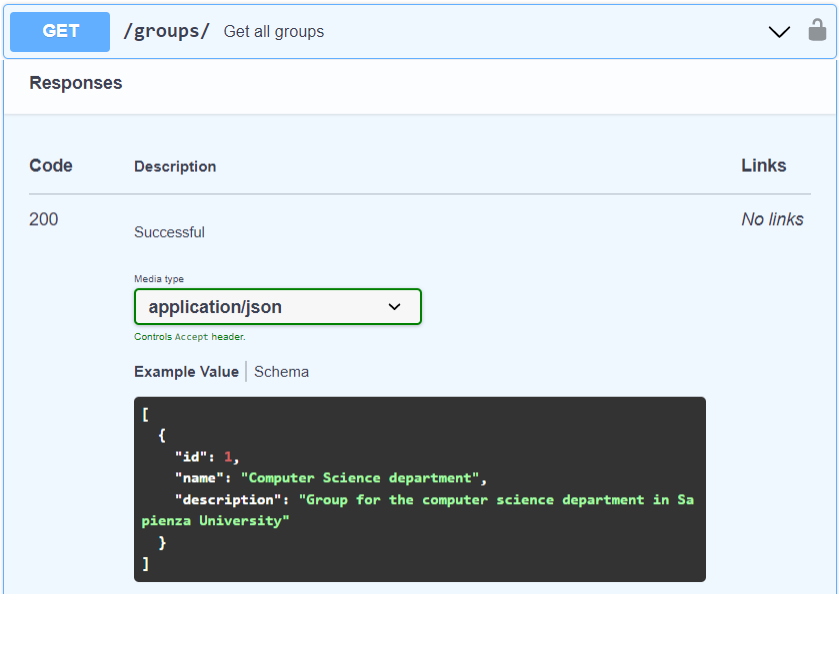
\includegraphics[width=1\linewidth]{img/add-link-task/groups.PNG}
    \caption{Groups API (GET)}
    \label{fig:groups}
\end{figure}
Una seconda idea, per ovviare ai problemi della prima, consiste nel creare questo identificativo univoco utilizzando un numero intero ed incrementarlo di una singola unità per ogni nuovo gruppo inserito nel database. Questo meccanismo può essere ottimizzato grazie al database usando la keyword \emph{autoincrement}. Il problema di questa implementazione è che l'ultimo ID univoco inserito permette di conoscere tutti gli altri identificativi precedenti; infatti, il numero dei gruppi esistenti, permetterà di conoscere gli identificativi utilizzati fino a quel momento (nonostante non si possa conoscere a priori il gruppo associato) e prevedere i prossimi ID inseriti.\newline
La soluzione finale è stata di generare casualmente un identificativo unico universale (UUID) tramite una libreria scritta in Go che permette di generare UUID v4 basato su numeri random (RFC-4122)\cite{UUID-library-documentation}. 
Lo UUID è composto da 16 byte (128 bit). Nella sua forma canonica, ed è rappresentato da 32 caratteri esadecimali, visualizzati in cinque gruppi separati da trattini, nella forma 8-4-4-4-12 per un totale di 36 caratteri (32 esadecimali e quattro trattini)\cite{GenerateUUID}\cite{rfc4122}. Perciò avremo \( 16^{32}=2^{128} \) combinazioni. Nella versione 4, 6 bit sono fissi e i restanti 122 bit sono generati casualmente, per un totale di \(2^{122}\) possibili UUID\cite{UUIDv4}, rendendo computazionalmente impossibile, in tempi umani, scoprire l'identificativo con un approccio di forza bruta. %Infatti, supponendo, per assurdo, che il tempo per richiedere l'accesso a un gruppo tramite invito impiegi 1 nanosecondo insieme al tempo di trasmissione e processamento della richiesta, questo vorrà dire che verranno impiegati \(\approx10940148113456098894032\approx 1.09\cdot10^{22}\) anni prima di trovare l'invitation id cercato, nel caso peggiore. Difatti abbiamo supposto una situazione completamente irreale e a favore dell'utente malevolo.
\newline
Nel caso l'identificativo di invito fosse ottenuto in qualsiasi altro modo da utenti malevoli, deve essere possibile poter sostituire il vecchio UUID con uno nuovo invalidando il precedente.
\newline
Quest'ultimo problema può essere risolto tramite la creazione di un nuovo endpoint API che sostituisce lo UUID.

\subsubsection{Database design}
Nella progettazione del database bisogna tenere conto di alcuni punti fondamentali:
\begin{itemize}
    \item Ogni gruppo deve avere un solo \emph{invitation id}
    \item Un \emph{invitation id} deve essere unico all'interno del database
    \item I gruppi creati in precedenza alle modifiche del database non avranno \emph{invitation id}, ma dovrà esserne generato uno se richiesto
    \item Ottimizzare accessi al database e alle tabelle
\end{itemize}
La prima soluzione è stata di creare una nuova tabella \say{groups\_invitations} (figura \ref{fig:invitation-first}) che lega il gruppo con il proprio \emph{invitation id}, dichiarandolo \say{\emph{unique}}.
\begin{figure}[H]
    \centering
    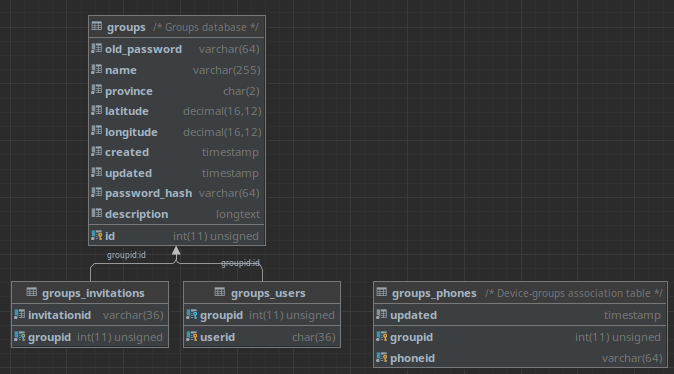
\includegraphics[width=1\linewidth]{img/add-link-task/invitation-first.png}
    \caption{Diagramma delle tabelle inerenti ai gruppi}
    \label{fig:invitation-first}
\end{figure}
Questo design permette di rispettare ogni punto precedente a costo di un ulteriore accesso in lettura per ottenere l'\emph{invitation id} del gruppo, nel caso servano anche le relative informazioni. Nonostante al momento non siano necessarie, per sviluppi futuri bisognerà offrire ulteriori informazioni oltre al semplice \emph{invitation id}. La retro compatibilità è garantita in quanto un gruppo che non possiede un \emph{invitation id} semplicemente non sarà presente nella tabella. L'unicità del \emph{invitation id} è garantita dal vincolo unique dichiarato durante la creazione della tabella.
\begin{figure}[H]
    \centering
    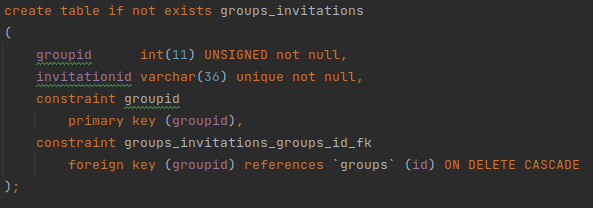
\includegraphics[width=1\linewidth]{img/add-link-task/invitation-first-code.png}
    \caption{Creazione tabella contenente gli \emph{invitation id}}
    \label{fig:invitation-first-code}
\end{figure}

E' stato preferito però un secondo design dello schema, ovvero accorpare la tabella \say{groups\_invitation} alla tabella \say{groups}, ottimizzando così gli accessi sia in lettura sia in scrittura. Si è aggiunta una nuova colonna \say{invitationid} (figure \ref{fig:invitation-final-code} e \ref{fig:invitation-final}) che contiene l'identificatore univoco dell'invito, il quale per mantenere la retro compatibilità potrà essere nullo. L'unicità dell'\emph{invitation id} è garantita dichiarando il parametro \say{unique}.

\begin{figure}[H]
    \centering
    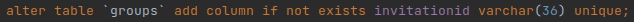
\includegraphics[width=1\linewidth]{img/add-link-task/invite-final.png}
    \caption{Modifica della tabella groups}
    \label{fig:invitation-final-code}
\end{figure}

\begin{figure}[H]
    \centering
    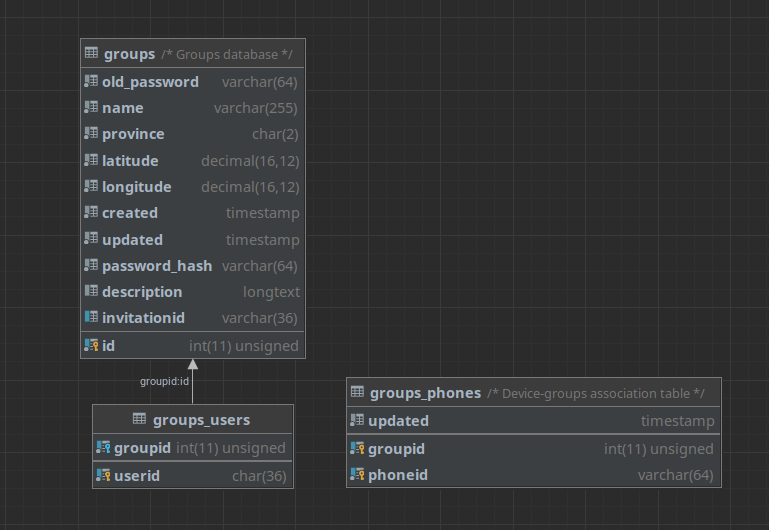
\includegraphics[width=1\linewidth]{img/add-link-task/invite-final-diagram.png}
    \caption{Diagramma finale della tabella groups}
    \label{fig:invitation-final}
\end{figure}


\subsubsection{API design}
Per la risoluzione del task è servito di creare 2 nuovi endpoint API \say{/me/group/invite}, \say{/me/group/redeeminvite} (figura \ref{fig:invite-redeem-group}) ed una per garantire la sicurezza dei gruppi \say{/me/group/updateinvite} (figura \ref{fig:update-invitation-id}).
\begin{figure}[H]
    \centering
    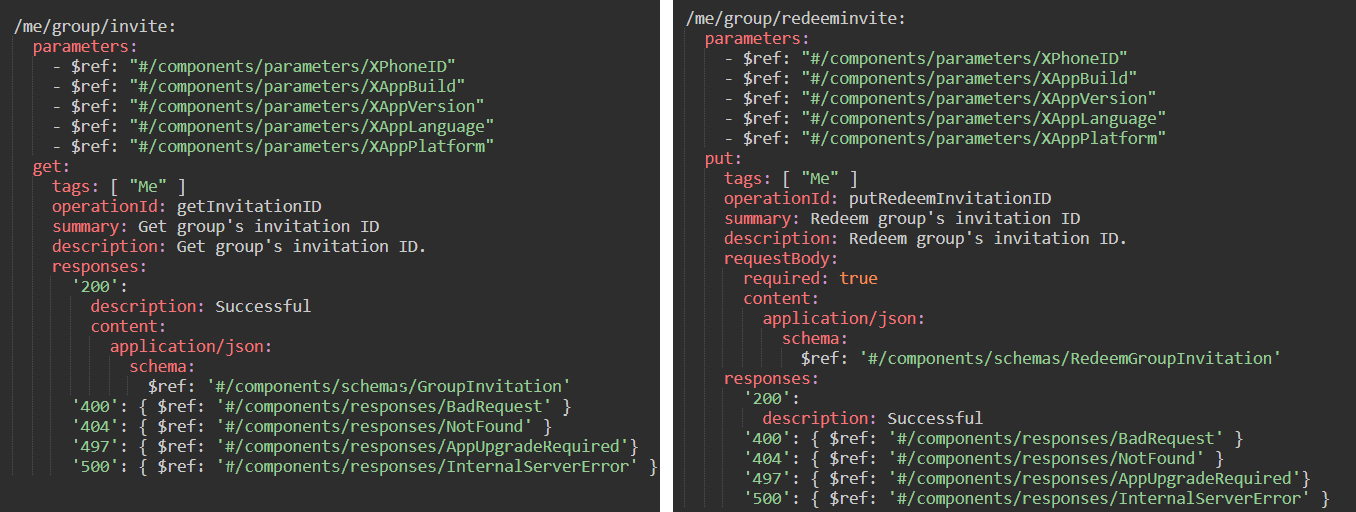
\includegraphics[width=1\linewidth]{img/add-link-task/invite-redeem-group-separated.png}
    \caption{Documentazione /me/group/invite e /me/group/redeeminvite}
    \label{fig:invite-redeem-group}
\end{figure}
\begin{figure}[H]
    \centering
    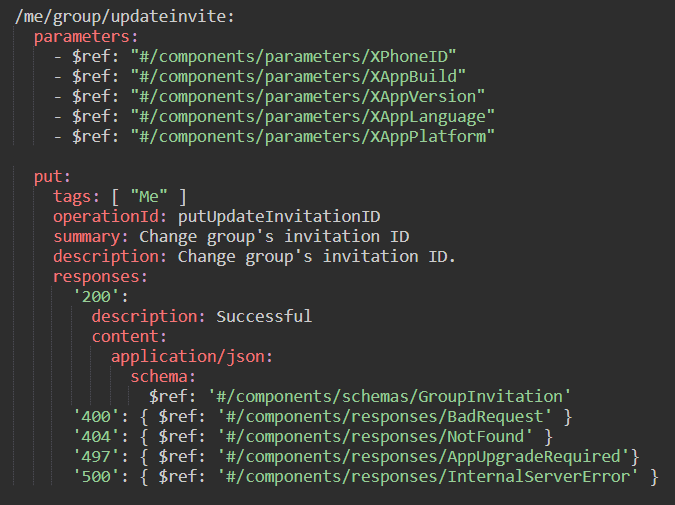
\includegraphics[width=1\linewidth]{img/add-link-task/update-invitation-id.png}
    \caption{Documentazione /me/group/updateinvite}
    \label{fig:update-invitation-id}
\end{figure}
Nell'API \say{/me/group/invite} viene raccolta la richiesta del client ritornando una risposta HTTP 200 insieme a un JSON contenente un oggetto \say{GroupInvitation}, il cui parametro è il codice di invito del gruppo a cui si appartiene (ritornare un oggetto aumenta la mantenibilità dell'endpoint in quanto si potranno aggiungere e rimuovere parametri modificando lo schema). Tutti i dati necessari, al soddisfacimento della richiesta, vengono raccolti dal database e processati per essere inseriti in un oggetto da ritornare in formato JSON.
\newline
Nell'API \say{/me/group/redeeminvite} il client richiede al server di essere aggiunto in un gruppo, passando l'\emph{invitation id} come parametro nel body della richiesta in formato JSON (come detto prima viene inviato un oggetto, si noti che è lo stesso del precedente endpoint, in modo da migliorare la mantenibilità).
\newline
Viene, quindi, interrogato il database per verificare che il client non faccia già parte di un gruppo e che il codice di invito esista. Passati i controlli si potrà inserire il client nel gruppo, aggiungendo un nuovo record all'interno del database, bypassando l'inserimento della password.
\newline
Nell'API \say{/me/group/updateinvite} viene generato un nuovo UUID v4 che verrà sostituito nella colonna \say{invitationid} presente nella tabella \say{groups} (figura \ref{fig:invitation-final}).
Quindi verrà modificato il campo solo nel gruppo in cui è presente l'utente che ne fa richiesta.


\subsubsection{Implementazione API}
\begin{figure}[H]
    \centering
    
\includegraphics[width=1\linewidth]{img/add-link-task/get-invite-API.PNG}
    \caption{Get-invite-API}
\end{figure}
\lstinputlisting[language=go]{Code/add-link-task/get-group-invitationid.go}

\begin{figure}[H]
    \centering
    
\includegraphics[width=1\linewidth]{img/add-link-task/redeem-invite-API.PNG}
    \caption{Redeem-invite-API}
\end{figure}
\lstinputlisting[language=go]{Code/add-link-task/redeem-invite-APi.go}

\begin{figure}[H]
    \centering
    
\includegraphics[width=1\linewidth]{img/add-link-task/update-invite-API.PNG}
    \caption{Update-invite-API}
\end{figure}
\lstinputlisting[language=go]{Code/add-link-task/update-invite-APi.go}


\end{document}

